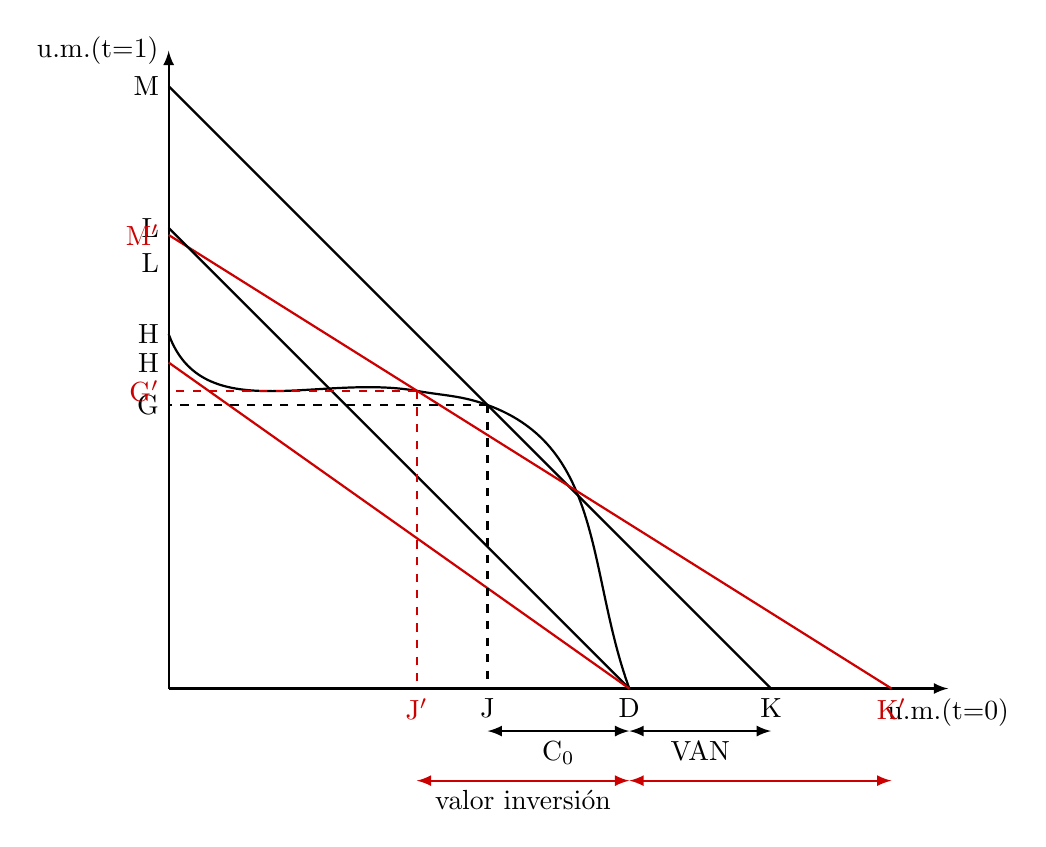
\begin{tikzpicture}[scale=0.9, >=latex]
  % Ejes
  \draw[->, thick] (0,0) -- (11,0) node[below] {u.m.(t=0)};
  \draw[->, thick] (0,0) -- (0,9) node[left] {u.m.(t=1)};

  % Puntos en el eje X
  % J' = 3.5, J = 4.5, D = 6.5, K = 8.5, K' = 10.0
  \coordinate (Jp) at (3.5,0);
  \coordinate (J) at (4.5,0);
  \coordinate (D) at (6.5,0);
  \coordinate (K) at (8.5,0);
  \coordinate (Kp) at (10.2,0);

  % Puntos en el eje Y
  % G = 4.0, G' = 4.5, H = 5.0, L = 6.0, M' = 6.25, M = 8.5 (approx, M' is intersection of red with Y, M is intersection of black with Y)
  % Actually we need points to match lines.
  % Black line: from (0, M) to (K, 0). (0, 8.5) to (8.5, 0). Slope = -1. Tangent at (J=4.5, G=4.0).
  % Wait, if slope is -1, 4.5+4.0 = 8.5. Matches!
  % So M = 8.5.
  \coordinate (M) at (0,8.5);
  % Red line: from (0, M') to (Kp, 0). (0, 6.25) to (10.2, 0). Tangent at J'=3.5. Let's find G'.
  % Slope = -6.25/10.2 = -0.6127.
  % At x=3.5, y = 6.25 - 0.6127*3.5 = 6.25 - 2.14 = 4.1. Let's call it G'=4.1.
  \coordinate (Mp) at (0,6.4);
  \coordinate (Gp) at (0,4.2);
  \coordinate (G)  at (0,4.0);

  % Draw opportunity curve: starts at D(6.5,0), passes through (4.5, 4.0) and (3.5, 4.2).
  \draw[thick] (6.5,0) to[out=110, in=-20] (4.5,4.0) to[out=160, in=-10] (3.5,4.2) to[out=170, in=-70] (0, 5.0);
  \node[left] at (0,5.0) {H};
  \node[left] at (0,6.0) {L};

  % Tangent lines
  % Black line
  \draw[thick] (M) -- (K);
  % Red line
  \draw[thick, red!80!black] (Mp) -- (Kp);

  % Another line from D to L? In the original PDF:
  % There's a black line from L on Y axis to D on X axis. This is the lending line without investment?
  % Yes, it represents the initial situation without investment? Or it represents the market line passing through D (endowment point).
  % If endowment is D, then market line 1 (black) passing through D has same slope as M-K.
  % Slope of M-K is -1. So line from D(6.5,0) with slope -1 goes to (0,6.5). Let's call L = 6.5.
  \draw[thick] (0,6.5) -- (D);
  \node[left] at (0,6.5) {L};

  % Market line 2 (red) passing through D has same slope as Mp-Kp.
  % Slope is -6.4/10.2 = -0.627. Line from D(6.5,0) goes to (0, 6.5*0.627) = 4.07. Wait, the point H is below L.
  \draw[thick, red!80!black] (0,4.6) -- (D); % Approximation
  \node[left] at (0,4.6) {H};

  % Fix M, M', G, G', J, J', K, K', D nodes
  \node[left] at (M) {M};
  \node[left, text=red!80!black] at (Mp) {M$'$};
  \node[left] at (G) {G};
  \node[left, text=red!80!black] at (Gp) {G$'$};

  \node[below] at (D) {D};
  \node[below] at (J) {J};
  \node[below, text=red!80!black] at (Jp) {J$'$};
  \node[below] at (K) {K};
  \node[below, text=red!80!black] at (Kp) {K$'$};

  % Dotted lines for tangency
  \draw[dashed, thick] (4.5,4.0) -- (4.5,0);
  \draw[dashed, thick] (4.5,4.0) -- (0,4.0);
  \draw[dashed, thick, red!80!black] (3.5,4.2) -- (3.5,0);
  \draw[dashed, thick, red!80!black] (3.5,4.2) -- (0,4.2);

  % Inversion arrows (C0)
  \draw[<->, thick] (4.5, -0.6) -- (6.5, -0.6) node[midway, below] {C$_0$};
  \draw[<->, thick] (6.5, -0.6) -- (8.5, -0.6) node[midway, below] {VAN};
  \draw[<->, thick, red!80!black] (3.5, -1.3) -- (6.5, -1.3);
  \draw[<->, thick, red!80!black] (6.5, -1.3) -- (10.2, -1.3);
  \node[below] at (5.0, -1.3) {valor inversión};
  % In original image, there is "valor inversión" bracket below the C0 bracket.
\end{tikzpicture}
